\subsection{Data Generation}
\label{sec:soft_cut_data_generation}

The raw data set from the 2007 TrecVid contest contains 1,592 soft cut frames and 637,755 non soft cut frames.
This is a highly imbalanced ratio, which impedes the training.
Also, the number of soft cuts in the data set is too small for training a deep neural net.
As stated by Greg Corrado, senior research scientist at Google: ``Training deep learning models really does take a lot of data''~\cite{dataDeepNeuralNets}.
Therefore, we generated more soft cuts by blending random sequences into each other.

The procedure for generating a new random sequence based on the data set provided by the 2007 TrecVid contest works as follows:
First, we randomly pick two subsequent cuts from the gold standard provided by the TrecVid contest, each with a start and end frame respectively.
Between the end frame of the first cut and the start frame of the next cut, we randomly select a subsequence with the desired transition length.
Because, there is no hard or soft cut between two subsequent cuts in the gold standard, it is guaranteed that there is also no hard or soft cut in the random sequence we picked.
Afterwards, we repeat this process with two other random cuts.
As the result, we now have two randomly selected sequences of the same length, which we now blend into each other.
In order to blend two random sequences, we have multiple options for tweening behaviour.
The standard tweening function is linear, but we also used ease-in, ease-out, and others. %, see Figure~\ref{fig:data_generation}.
The tweening function is randomly selected, as well.
As the transition type we use a classic \textit{dissolve}.
In order to achieve further variance in the generated data, we flip the two sequences randomly at the x- or y-axis or at both axes.
With this approach we generated about 50 GB of data.
% \textcolor{red}{TODO}: Das ist ja jetzt gerade unvergleichbar mit den Zahlen von oben, weil wir oben absolute Zahlen hatten und hier auf einmal GB.
% Das muessen wir noch vereinheitlichen.
% ICh bin dafuer, hier noch die Anzahl der Soft cuts/non soft cuts hinzuschreiben.

% \begin{figure}[ht]
%     \centering
%     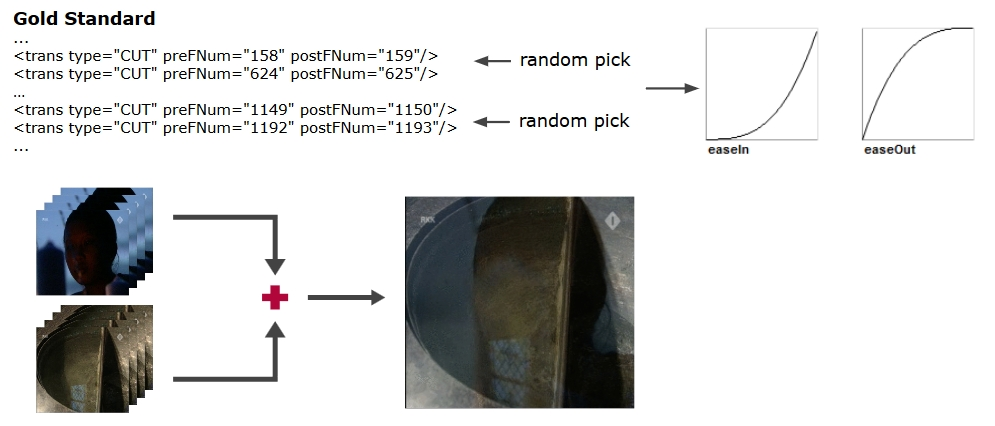
\includegraphics[scale=.5]{images/data_generation.jpg}
%     \caption{}
%     \label{fig:data_generation}
% \end{figure}
% \textcolor{red}{TODO}: Figure Text missing.
